\chapter{DESENVOLVIMENTO DO PROTÓTIPO}
\label{cap:desenvolvimento}

Este capítulo descreve a arquitetura e a implementação do protótipo. Primeiro, apresenta-se a visão geral da solução final; em seguida, cada componente é detalhado: a base local da tabela NCM, a detecção de produtos com NCM inválido, o processo de sugestão, a base de conhecimento formada por produtos de outras empresas, a verificação de produtos com NCM possivelmente incorreto, a execução em segundo plano e a interface de supervisão. Ao final, descreve-se a evolução das versões testadas ao longo do trabalho, incluindo as que foram descartadas e os motivos.

\section{Visão Geral da Arquitetura}

A Figura~\ref{fig:arquitetura_final} apresenta a arquitetura final. O protótipo é uma aplicação independente do ERP, que se conecta ao mesmo banco de dados Firebird e não exige nenhuma alteração no código-fonte do Lux Auto. Um processo em segundo plano consulta periodicamente o banco e identifica produtos com NCM inválido; em lotes menores, também verifica produtos com NCM válido, em busca de códigos que existem, mas parecem pertencer a outro tipo de produto. Para cada produto, o processo de sugestão consulta a base local com a tabela NCM, a base de conhecimento com produtos já classificados por outras empresas e o modelo de linguagem, executado pelo Ollama, e grava as três opções mais prováveis em um cache local. O operador é avisado por uma notificação do Windows e, na interface Streamlit, escolhe uma das opções; somente então o NCM é gravado no cadastro do produto.

\begin{figure}[H]
    \centering
    \caption{Arquitetura final do protótipo}
    \label{fig:arquitetura_final}
    \begin{tikzpicture}[
        node distance=0.9cm and 1.3cm,
        every node/.style={font=\small},
        box/.style={rectangle, draw, rounded corners=4pt, minimum height=1cm, align=center, fill=blue!8, text width=4.2cm},
        dado/.style={rectangle, draw, rounded corners=4pt, minimum height=1cm, align=center, fill=yellow!15, text width=4.2cm},
        userbox/.style={rectangle, draw, rounded corners=4pt, minimum height=1cm, align=center, fill=green!10, text width=4.2cm},
        arrow/.style={-{Stealth[scale=1]}, thick}
    ]
        \node (erp)     [dado] {Banco do ERP Lux Auto\\(Firebird)};
        \node (worker)  [box, below=of erp] {Processo em segundo plano\\(detecção e verificação)};
        \node (sug)     [box, below=of worker] {Sugestão de NCM\\(busca + escolha)};
        \node (cache)   [dado, below=of sug] {Cache de sugestões\\(SQLite)};
        \node (ui)      [box, below=of cache] {Interface de supervisão\\(Streamlit) e notificação};
        \node (ncm)     [dado, right=2.2cm of worker] {Tabela NCM e base de conhecimento (SQLite + FTS5)};
        \node (llm)     [box, right=2.2cm of cache] {Modelo de linguagem\\(Ollama, Qwen3 8B)};
        \node (user)    [userbox, right=2.2cm of ui] {Operador\\(\textit{Human-in-the-Loop})};

        \draw [arrow] (erp) -- node[right, font=\footnotesize] {SELECT} (worker);
        \draw [arrow] (worker) -- node[right, font=\footnotesize] {inválido ou suspeito} (sug);
        \draw [arrow, <->] (sug.east) -- node[above, sloped, font=\footnotesize] {candidatos} (ncm.south west);
        \draw [arrow, <->] (sug.east) -- node[below, sloped, font=\footnotesize] {escolhas} (llm.north west);
        \draw [arrow] (sug) -- node[right, font=\footnotesize] {3 opções} (cache);
        \draw [arrow] (cache) -- (ui);
        \draw [arrow, <->] (ui) -- node[above, font=\footnotesize] {escolhe} (user);
        \draw [arrow] (ui.west) -- ++(-0.8,0) |- node[left, pos=0.25, font=\footnotesize, align=center] {UPDATE\\aprovado} (erp.west);
    \end{tikzpicture}
    \fonte{O autor (2026).}
\end{figure}

Em relação à arquitetura prevista no projeto, a principal mudança é o papel do modelo de linguagem. No projeto, o agente receberia a estrutura do banco e geraria consultas SQL a partir de instruções em linguagem natural (\textit{Text-to-SQL}). Na solução final, todas as consultas SQL são fixas e parametrizadas, escritas no código, e o modelo não tem acesso ao banco: ele recebe apenas a descrição do produto e uma lista de códigos candidatos, e sua resposta é restrita, por esquema JSON, a escolher entre esses códigos. A seção~\ref{sec:evolucao} explica como se chegou a essa decisão. O fluxo de aprovação humana previsto no projeto foi mantido integralmente.

\section{Base Local da Tabela NCM}

A tabela NCM vigente foi obtida em formato PDF, com 505 páginas, e extraída para um banco SQLite com a biblioteca pdfplumber, resultando em 15.141 linhas, que abrangem todos os níveis da hierarquia, dos capítulos aos itens. Durante a extração, observou-se que, em parte das linhas, uma camada de texto sobreposta no PDF fazia os caracteres da data de vigência se intercalarem com o final da descrição. Como a ordem relativa dos caracteres de cada campo se preserva nessa intercalação, um script de reparo separou os dígitos que formam a data do restante do texto e reconstruiu a descrição. Algumas descrições ainda apresentam pequenos defeitos herdados da extração, como palavras emendadas.

Essa base resolveu um problema prático observado no início do trabalho: tentar fornecer a tabela inteira a um modelo de linguagem excede qualquer janela de contexto viável. Com a base local, a validação de um código passa a ser uma consulta direta, e o modelo recebe apenas algumas dezenas de candidatos relevantes, no espírito da RAG descrita na seção~\ref{sec:recuperacao}.

Para a busca, foi construído um índice de texto completo (FTS5) somente sobre os 10.504 códigos de oito dígitos, já que apenas eles são válidos no cadastro. Como a descrição de um item frequentemente só faz sentido com os níveis superiores (seção~\ref{sec:ncm}), cada item foi indexado com três colunas: o texto próprio do item; o texto de todos os seus ancestrais (capítulo, posição e subposições); e uma versão do texto sem hífens. A primeira coluna recebe peso maior no BM25 (5,0, contra 1,0 dos ancestrais e 0,5 da versão sem hífen), de modo que um item cujo próprio texto corresponde à busca fique à frente de um item que só corresponde pelo cabeçalho. A coluna sem hífen permite que descrições digitadas sem hífen, como ``PARACHOQUE'', encontrem ``para-choques''. O índice ignora acentos, o que torna a busca tolerante a descrições digitadas sem acentuação.

\section{Detecção de Produtos com NCM Inválido}

A detecção não utiliza o modelo de linguagem. Uma consulta somente leitura obtém todos os produtos cadastrados como mercadoria (campo \texttt{SERVICO = 'N'}), excluindo os serviços, cujo campo NCM guarda um código NBS (seção~\ref{sec:ncm}). Para cada produto, o código cadastrado é normalizado (o ERP grava os oito dígitos sem pontuação) e considerado inválido quando está vazio, não possui oito dígitos ou não existe na tabela vigente. Por ser uma regra determinística, a detecção não está sujeita a alucinação e executa em milissegundos.

Essa regra detecta códigos vazios, malformados, inexistentes ou extintos em atualizações da tabela, que são os que causam rejeição imediata da NF-e por código inválido. Ela não detecta um produto cadastrado com um código válido, porém de outro produto, por exemplo um parafuso classificado como pneu; esse tipo de erro exige comparar a descrição do produto com o texto do código cadastrado e é tratado pela verificação descrita na seção~\ref{sec:verificacao}.

\section{Sugestão da Classificação}
\label{sec:sugestao}

O processo de sugestão recebe a descrição do produto e devolve até três códigos NCM, do mais para o menos provável, cada um com uma justificativa curta. A Figura~\ref{fig:pipeline_sugestao} resume suas etapas, detalhadas a seguir.

\begin{figure}[H]
    \centering
    \caption{Etapas da sugestão de NCM na versão final}
    \label{fig:pipeline_sugestao}
    \begin{tikzpicture}[
        node distance=0.55cm,
        every node/.style={font=\small},
        box/.style={rectangle, draw, rounded corners=4pt, align=left, fill=blue!8, text width=11.5cm, minimum height=0.9cm},
        llmbox/.style={rectangle, draw, rounded corners=4pt, align=left, fill=orange!15, text width=11.5cm, minimum height=0.9cm},
        arrow/.style={-{Stealth[scale=1]}, thick}
    ]
        \node (e0) [box] {\textbf{Entrada:} descrição do produto, como cadastrada (ex.: ``PASTILHA FREIO DIANT GOL'')};
        \node (e1) [box, below=of e0] {\textbf{1. Abreviações e memória:} expansão das abreviações do cadastro e produtos parecidos já classificados no próprio ERP};
        \node (e2) [llmbox, below=of e1] {\textbf{2. Análise (LLM):} descrição técnica no vocabulário da NCM e características que decidem a classificação};
        \node (e3) [box, below=of e2] {\textbf{3. Busca:} FTS5/BM25 + sinônimos, pela descrição original e pela técnica, fundidas por RRF, mais os NCMs mais votados na base de conhecimento};
        \node (e4) [llmbox, below=of e3] {\textbf{4. Escolha do capítulo (LLM):} entre os capítulos dos candidatos, ou ``nenhum''};
        \node (e5) [llmbox, below=of e4] {\textbf{5. Escolha dos itens (LLM):} as 3 opções mais prováveis no capítulo e a informação que falta, se houver};
        \node (e6) [box, below=of e5] {\textbf{6. Voto da base de conhecimento:} quando a base é confiante, seu NCM mais votado passa ao 1º lugar};
        \node (e7) [box, below=of e6] {\textbf{Saída:} 3 opções com justificativa, pergunta ao operador e produtos parecidos};

        \foreach \a/\b in {e0/e1, e1/e2, e2/e3, e3/e4, e4/e5, e5/e6, e6/e7} \draw [arrow] (\a) -- (\b);
    \end{tikzpicture}
    \fonte{O autor (2026). Em laranja, as etapas que consultam o modelo de linguagem.}
\end{figure}

\subsection{Memória de Classificações}

Em uma oficina, um produto novo quase sempre se parece com algum já cadastrado, como ``PASTILHA FREIO DIANT GOL'' e ``PASTILHA FREIO TRAS PALIO''. O NCM que a empresa já usa para o produto parecido é a pista mais forte disponível, pois reflete como aquela empresa classifica seus produtos. Por isso, a primeira etapa procura, entre os produtos do próprio ERP que já possuem NCM válido, aqueles com descrição semelhante. A semelhança entre os conjuntos de palavras $A$ e $B$ das duas descrições, sem acentos e sem palavras genéricas, é calculada como a média entre o coeficiente de Jaccard (seção~\ref{sec:knn}) e a sobreposição relativa ao menor conjunto \cite{manning2008ir}:

\begin{equation}
\label{eq:similaridade}
\mathrm{sim}(A, B) = \frac{1}{2}\,\frac{|A \cap B|}{|A \cup B|} + \frac{1}{2}\,\frac{|A \cap B|}{\min(|A|, |B|)}
\end{equation}

O segundo termo foi incluído porque o Jaccard sozinho penaliza o caso mais comum em cadastros, em que uma descrição está contida na outra (``PARACHOQUE'' e ``PARACHOQUE DIANTEIRO GOL''). Produtos com semelhança a partir de 0,4 são considerados parecidos. O código do mais parecido é inserido no topo da lista de candidatos, e até três produtos parecidos são informados ao modelo como indício a ser conferido. Como as aprovações feitas na interface gravam o NCM no próprio cadastro, essa memória cresce com o uso, sem exigir nenhuma tabela adicional.

\subsection{Expansão de Abreviações}

As descrições digitadas no ERP são, com frequência, abreviadas: ``PIVO SUSP INF DIANT'' é um pivô da suspensão inferior dianteira. Nos primeiros testes da segunda fase, abreviações levaram o modelo a interpretações absurdas, como ``SUSP INF'' lida como ``medicamento para infusão''. Por isso, antes de qualquer outra etapa, as abreviações mais comuns do setor são expandidas por uma tabela com 85 entradas (por exemplo, ``DIANT'' para ``dianteiro'', ``JG'' para ``jogo'' e ``ROLAM'' para ``rolamento''). Abreviações ambíguas, como ``PC'' (peça ou computador) e ``DIA'', foram mantidas fora da tabela. A descrição expandida é mostrada ao modelo ao lado da original, que é preservada para a busca.

\subsection{Análise do Produto}

A tabela NCM raramente usa o nome comercial do produto. A segunda etapa pede ao modelo de linguagem que reescreva a descrição com o nome técnico usado pela NCM, em no máximo oito palavras e sem embalagem, medidas ou marca, e que liste as características que decidem a classificação, como material, função, aplicação e se o produto é completo ou uma peça. Quando algo importante não pode ser inferido da descrição, o modelo deve indicá-lo como ``não informado''. O \textit{prompt}, reproduzido no Apêndice~\ref{ap:prompts}, traz três exemplos de produtos que não fazem parte de nenhum conjunto de avaliação.

\subsection{Busca de Candidatos}

A busca é executada duas vezes, uma com a descrição original e outra com a descrição técnica, e as duas listas são combinadas por fusão de rankings (RRF, Equação~\ref{eq:rrf}, com $k = 60$), resultando em até 40 candidatos. A esses candidatos somam-se, no topo da lista, os NCMs mais votados na base de conhecimento (seção~\ref{sec:conhecimento}), quando houver. A descrição original preserva termos que o modelo pode descartar indevidamente; a técnica traz o vocabulário da tabela.

Antes de consultar o índice, cada descrição passa por um tratamento: extraem-se apenas as palavras com três letras ou mais, o que também descarta números e medidas como ``195/65'' e ``500ML''; removem-se palavras genéricas que aparecem em milhares de itens, como ``tipo'', ``uso'', ``embalagem'' e ``unidade''; e cada palavra é buscada como prefixo, entre aspas, o que neutraliza caracteres e palavras reservadas da sintaxe de busca. A busca por prefixo cobre a maioria dos plurais, mas não os irregulares, como ``farol'' e ``faróis''; para esses casos, o plural é gerado por regras simples de sufixo e acrescentado à consulta.

Quando uma palavra da descrição não encontra nenhum item na tabela, seus sinônimos são obtidos da OpenWordNet-PT, por meio da NLTK, e buscados em uma consulta separada, que ocupa uma pequena reserva de posições na lista. A consulta é separada porque, nos testes, misturar sinônimos de palavras comuns na consulta principal gerava ruído excessivo. Uma pequena lista manual complementa a WordNet em casos observados, como ``azulejo'', cujo termo oficial é ``ladrilho''.

\subsection{Escolhas Restritas do Modelo}

Com os candidatos em mãos, o modelo de linguagem faz duas escolhas curtas. Na primeira, os candidatos são agrupados por capítulo e apresentados em ordem de relevância, cada capítulo com seu título e alguns itens resumidos, e o modelo indica a qual capítulo o produto pertence ou responde ``NENHUM'', se nenhum for do mesmo tipo de produto. Na segunda, o modelo recebe apenas os itens do capítulo escolhido, com o caminho completo de cada um, e devolve os três mais prováveis, em ordem, com uma justificativa curta, além da informação que falta para decidir, se houver. Essa informação é apresentada ao operador como uma pergunta, por exemplo ``O valor Brix do suco de uva é superior ou igual a 30?''.

As duas respostas são restritas por esquema JSON (seção~\ref{sec:recuperacao}): o campo do capítulo só aceita os capítulos apresentados, e o campo de código só aceita os códigos apresentados. Assim, o modelo não consegue inventar um código inexistente nem escapar do formato esperado. O esquema da segunda escolha é ilustrado a seguir, com a lista de códigos abreviada:

{\small
\begin{verbatim}
{"type": "object",
 "properties": {
   "opcoes": {"type": "array", "minItems": 1, "maxItems": 3,
     "items": {"type": "object",
       "properties": {
         "justificativa": {"type": "string"},
         "codigo": {"type": "string",
                    "enum": ["8708.30.11", "8708.30.19", ...]}},
       "required": ["justificativa", "codigo"]}},
   "informacao_que_falta": {"type": "string"}},
 "required": ["opcoes", "informacao_que_falta"]}
\end{verbatim}
}

O \textit{prompt} de sistema que acompanha as duas escolhas (Apêndice~\ref{ap:prompts}) orienta o modelo a pensar no que o produto é de fato antes de escolher, a não se deixar levar por palavras soltas como a cor, a evitar itens ``Outros'' por insegurança e, como desempate, a preferir a aplicação automotiva quando a descrição não diz o tipo de veículo, já que o ERP atende oficinas mecânicas. Na segunda fase, acrescentou-se ao \textit{prompt} a Nota 2 da Seção XVII (seção~\ref{sec:ncm}): no conjunto de desenvolvimento, peças de uso geral, como rolamentos, mangueiras e palhetas, eram classificadas como ``partes e acessórios'' de veículos (posição 87.08), e a regra lista as posições próprias dessas peças. Trata-se de uma regra oficial da tabela, e não de um ajuste caso a caso.

Dois tratamentos adicionais se mostraram necessários. O primeiro é a tradução de referências cruzadas: o texto oficial cita outras posições apenas pelo número, como em ``partes e acessórios dos veículos das posições 87.11 a 87.13'', e o modelo não tem como saber que essas posições são motocicletas, bicicletas e cadeiras de rodas. Sem essa informação, pastilhas de freio de carro eram classificadas como peças de bicicleta; por isso, o nome curto de cada posição citada é acrescentado ao texto. O segundo é a validação da resposta: os modelos Qwen eventualmente inserem palavras em chinês no meio de respostas em português, e esses trechos são removidos; além disso, se a resposta vier fora do formato, a pergunta é repetida uma vez. Se o modelo devolver menos de três opções, a lista é completada com os próximos itens do capítulo na ordem da busca, identificados como alternativas sem análise do modelo.

\section{Base de Conhecimento de Outras Empresas}
\label{sec:conhecimento}

A memória de classificações depende de o próprio ERP já ter produtos parecidos classificados, o que não ocorre em uma instalação nova. Para suprir essa falta, foi construída uma base de conhecimento com os produtos já classificados por outras empresas do mesmo setor, a partir das bases cedidas por duas lojas de autopeças (Capítulo~\ref{cap:metodologia}). Não se trata de treinar o modelo de linguagem, o que exigiria mais memória de vídeo do que a disponível, mas de uma classificação por vizinhos mais próximos (seção~\ref{sec:knn}): para um produto novo, buscam-se os dez produtos mais parecidos já classificados, e cada um vota no seu NCM com peso $1/(1+i)$, em que $i$ é sua posição na lista, a partir de zero.

A semelhança é dada pela busca BM25 sobre os radicais das palavras da descrição, obtidos pelo algoritmo Snowball para o português, depois da expansão de abreviações. Antes da indexação, remove-se o prefixo com a marca e o código do fabricante, frequente nas descrições do setor (``VIEMAR 680077 - ARTICULADOR AXIAL DIRECAO''), que identifica o fabricante, e não o tipo de produto.

Uma base de exemplos herda os erros de quem a produziu. Na Loja B, o código 8708.10.00 (para-choques) aparece em 3.407 produtos, dos quais apenas 104 são para-choques; os demais são molas, freios, cabos e rolamentos, cadastrados com um código ``coringa''. Por isso, produtos com esse código cuja descrição não menciona para-choque são excluídos da base. A mesma situação foi aproveitada como caso real para avaliar a detecção de NCM incorreto (Capítulo~\ref{cap:resultados}).

A base é usada de três formas no processo de sugestão: os NCMs mais votados entram no topo da lista de candidatos; até cinco produtos parecidos são mostrados ao modelo como indício; e, depois da escolha do modelo, se o NCM mais votado tiver voto de pelo menos 2,0 e o vizinho mais próximo for bastante parecido, esse NCM passa ao primeiro lugar, com a justificativa de que outras lojas classificam produtos parecidos dessa forma. Os limiares foram definidos no conjunto de desenvolvimento.

\section{Verificação de NCM Possivelmente Incorreto}
\label{sec:verificacao}

Um código válido pode pertencer a outro produto. Para apontar esses casos, o protótipo verifica produtos com NCM válido combinando dois sinais. O primeiro é a própria sugestão: o processo da seção~\ref{sec:sugestao} é executado para o produto, como se ele não tivesse NCM, e verifica-se se o código cadastrado está entre as três opções sugeridas. O segundo é um veredito do modelo sobre o código cadastrado: o modelo recebe a descrição do produto e o texto oficial completo do código, do capítulo ao item, e responde, com resposta restrita por esquema JSON, se o texto descreve esse tipo de produto (``compatível''), outro tipo de produto (``incompatível'') ou se depende de uma informação ausente (``dúvida'').

O produto é apontado como possivelmente incorreto somente quando os dois sinais concordam: o código cadastrado está fora das três opções sugeridas e o modelo o considera incompatível. Outras combinações foram avaliadas, como uma comparação lado a lado entre o código cadastrado e as opções sugeridas, apresentadas em ordem aleatória, e o voto da base de conhecimento; a regra final foi escolhida no conjunto de desenvolvimento por apresentar a melhor combinação entre detecção e alarmes falsos (Capítulo~\ref{cap:resultados}). Para não confundir uma suspeita com um erro, a interface apresenta a decisão como ``NCM possivelmente errado'', com o motivo e as opções sugeridas, e a decisão final é sempre do operador.

\section{Execução em Segundo Plano e Notificação}

Para que a sugestão já esteja pronta quando o operador a procurar, um processo em segundo plano consulta o banco a cada 20 segundos, identifica produtos com NCM inválido ainda sem sugestão e executa o processo de sugestão para cada um. Em seguida, verifica um pequeno lote de produtos com NCM válido, dos cadastrados mais recentemente para os mais antigos, de modo que a verificação de um cadastro inteiro avance aos poucos sem atrasar as sugestões dos produtos com NCM inválido. O resultado é gravado em um cache SQLite local, separado do banco do ERP, cuja chave é o par código do produto e descrição: se o operador corrigir a descrição no ERP, a sugestão antiga deixa de valer e é recalculada. Ao concluir cada produto, o processo pode exibir uma notificação do Windows com a primeira opção sugerida.

Optou-se pela consulta periódica (\textit{polling}) em vez de um gatilho (\textit{trigger}) no banco porque um gatilho exigiria alterar a estrutura do banco do ERP em cada cliente, contrariando a premissa de não modificar o sistema principal. O custo é um atraso de até 20 segundos para o produto ser notado, além do tempo de sugestão.

\section{Interface de Supervisão}

A interface, desenvolvida em Streamlit, lista os produtos com NCM inválido e, para cada um, exibe as opções sugeridas, como ilustra a Figura~\ref{fig:tela_streamlit}. Acima das opções, são apresentadas a interpretação feita pelo modelo, as características consideradas, os produtos parecidos já cadastrados e, quando houver, a pergunta sobre a informação que falta. O operador escolhe uma das três opções e confirma; somente nesse momento o sistema executa a atualização do cadastro. Se nenhuma opção servir, o operador pode descartar a sugestão e pedir uma nova. Uma segunda seção da interface lista os produtos com NCM possivelmente errado, com o código cadastrado, o motivo da suspeita e as opções sugeridas; o operador pode trocar o código por uma das opções ou indicar que o código atual está correto, e, nesse caso, o produto deixa de ser apontado.

\begin{figure}[H]
    \centering
    \caption{Interface de supervisão com as opções sugeridas para um produto}
    \label{fig:tela_streamlit}
    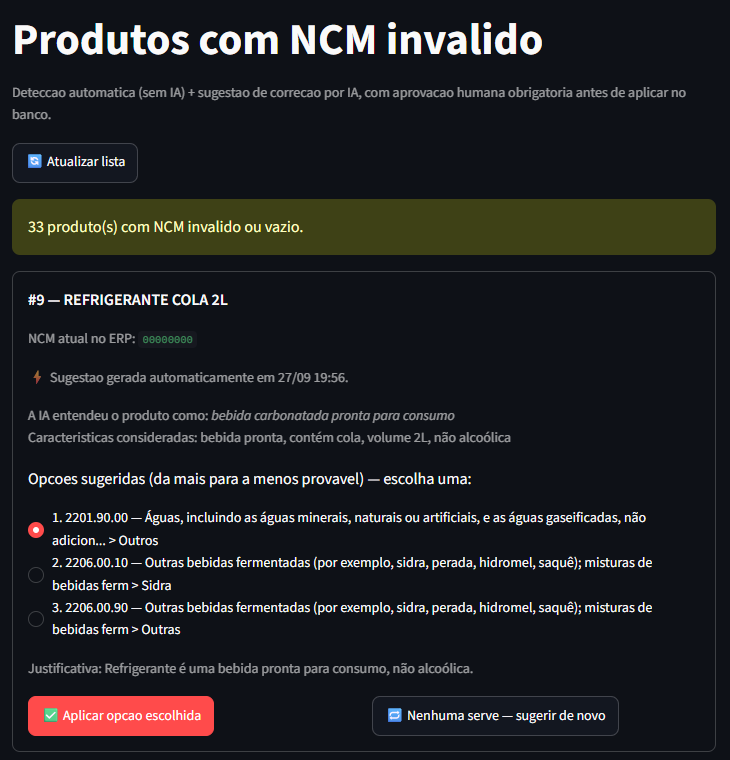
\includegraphics[width=11cm]{images/tela_streamlit.png}
    \fonte{O autor (2026).}
\end{figure}

O exemplo da Figura~\ref{fig:tela_streamlit} é um dos erros do conjunto de teste: para um refrigerante de cola, as três opções sugeridas são de águas e de bebidas fermentadas, e não a posição correta, de bebidas não alcoólicas (2202.10.00). É justamente para esse tipo de caso que a aprovação humana existe: o operador percebe que nenhuma opção corresponde ao produto e, em vez de aplicar a sugestão, pede uma nova ou classifica o produto manualmente.

A camada de acesso ao banco impõe duas restrições. Toda consulta de leitura passa por uma função que só aceita comandos \texttt{SELECT}. A gravação passa por outra função, que só aceita comandos \texttt{UPDATE} com parâmetros, e é chamada apenas pelo botão de aprovação da interface, com um comando fixo: \texttt{UPDATE PRODUTO SET NCM = ? WHERE CODIGO = ?}. Como o código gravado é sempre um dos códigos existentes na tabela, apresentados ao operador, não há como o sistema gravar um código inventado. Por controlar alterações no banco de produção, a interface é servida apenas para o próprio computador (\textit{localhost}).

\section{Evolução das Versões}
\label{sec:evolucao}

A arquitetura final resultou de uma sequência de versões, cada uma motivada pelos erros da anterior. O Quadro~\ref{qua:versoes} resume essa evolução; os resultados quantitativos são apresentados no Capítulo~\ref{cap:resultados}.

\begin{quadro}[H]
\centering
\caption{Versões do processo de sugestão avaliadas}
\label{qua:versoes}
\begin{tabular}{|p{3.3cm}|p{6.2cm}|p{4.7cm}|}
\hline
\textbf{Versão} & \textbf{Funcionamento} & \textbf{Situação} \\
\hline
Agente com ferramentas & LLM decide quais ferramentas chamar (busca na tabela, listagem de subcódigos, consulta ao banco) e em que ordem & Descartada: lenta, instável e com alucinações \\
\hline
Busca com \textit{embeddings} & Busca semântica por vetores somada à busca lexical & Descartada: não aproximou o vocabulário comercial do técnico \\
\hline
Busca e escolha & Busca lexical e duas escolhas restritas do LLM; primeiro com uma opção, depois com três & Base da versão final \\
\hline
Navegação hierárquica & LLM navega capítulo, posição e item vendo a lista completa de cada nível & Descartada: mais lenta e menos precisa \\
\hline
Busca e escolha revisada (1ª fase) & Busca e escolha, com análise do produto, pergunta ao operador, memória e nova tentativa & Base da segunda fase \\
\hline
Dicas de posição e hipóteses & LLM sugere posições prováveis e interpretações alternativas, buscadas também & Descartadas: pioraram ou não alteraram o acerto \\
\hline
Final (2ª fase) & Busca e escolha revisada, com Qwen3 8B, expansão de abreviações, Nota 2 da Seção XVII e base de conhecimento & Adotada \\
\hline
\end{tabular}
\fonte{O autor (2026).}
\end{quadro}

A primeira versão seguiu o projeto: um agente LangChain com o Llama 3.1 8B, que recebia ferramentas para consultar o banco do ERP e a tabela NCM e decidia, em várias rodadas, quais chamar. Na prática, cada classificação exigia de três a cinco chamadas sequenciais ao modelo, o que tornava a resposta lenta e expunha a instabilidade do servidor local sob uso repetido. Mais grave, o modelo nem sempre usava as ferramentas como instruído: em um dos testes, classificou um azulejo de banheiro como ``tubo de escape'', código que não tinha relação com nenhum resultado de busca. Esse comportamento levou à decisão de inverter o controle: o programa executa a busca de forma determinística e o modelo apenas escolhe, com a resposta restrita aos candidatos.

Em paralelo, testou-se a busca semântica com dois modelos de \textit{embeddings} (nomic-embed-text e paraphrase-multilingual-mpnet-base-v2), para encontrar itens sem palavras em comum com a descrição. Os vetores não aproximaram de forma útil o vocabulário comercial do técnico (``azulejo'' de ``ladrilho'', ``bateria'' de ``acumulador''), e o uso de um segundo modelo obrigava o Ollama a alternar modelos na memória de vídeo a cada sugestão, o que travava o servidor. A expansão por sinônimos da WordNet, mais simples, foi adotada no lugar.

A versão de busca e escolha inicialmente devolvia uma única opção. A análise de erros mostrou que, quando o modelo errava, a resposta certa costumava estar entre os primeiros candidatos do mesmo capítulo (leite integral e desnatado, pilha AA e C), o que motivou a apresentação de três opções ao operador.

A navegação hierárquica foi testada para eliminar a dependência da busca: em vez de escolher entre candidatos, o modelo via a lista completa dos 96 capítulos, depois todas as posições do capítulo escolhido e, por fim, todos os itens das posições escolhidas, como faria um classificador humano seguindo as Regras Gerais de Interpretação. Apesar de acertar o capítulo com frequência, essa versão errou mais na escolha final e foi mais lenta, como mostra o Capítulo~\ref{cap:resultados}. A primeira fase terminou com o retorno à busca e escolha, incorporando as melhorias que funcionam independentemente da forma de navegação: a análise do produto com características, a pergunta ao operador, a memória de classificações e a nova tentativa em caso de resposta fora do formato.

A segunda fase partiu dessa versão e foi conduzida sobre os conjuntos de desenvolvimento dev e DEV2. A análise dos erros no DEV2 mostrou três problemas principais: abreviações mal interpretadas, peças de uso geral classificadas como partes de veículos e o código correto ausente dos candidatos. Os dois primeiros motivaram a expansão de abreviações e a inclusão da Nota 2 da Seção XVII. Para o terceiro, foram testadas duas formas de dar ao modelo mais candidatos: pedir a ele as posições de quatro dígitos mais prováveis, cujos itens eram acrescentados à lista, e pedir interpretações alternativas do produto, buscadas também. Ambas pioraram ou não alteraram o acerto e foram descartadas. O modelo Qwen3 8B, disponível nessa fase, substituiu o Qwen2.5 7B por interpretar melhor os produtos (``água sanitária'' passou a ser reconhecida como produto de desinfecção, e ``serrote'', como ferramenta de corte de madeira). Por fim, a base de conhecimento das duas lojas permitiu tratar a falta de candidatos e a escolha fina nos produtos automotivos, que são o foco do ERP.
